\chapter{Introduction}

Software is increasingly complex with many interactions among
different pieces of software and the operating system.
The complex interactions make the software ecosystem hard to understand.
Without proper understanding,
it is difficult to configure/maintain software and to fix problems.
The complexity also increases the attack surface\cite{manadhata2006attack}, which measures the
bugs or features exploitable by malicious attacks.
Monitoring is an effective way to understand these interactions.
Software monitoring is the process of obtaining information
in running software.
It is used for different purposes and the information obtained is different
according to the purpose:

\begin{itemize}
\item {\bf software comprehension} \\
Monitoring can help software comprehension such as studying the control
flow and module dependency.
Monitoring running software can be used to study the dynamic behaviour which
cannot be achieved from static analysis.
\item {\bf verification} \\
We can observe the expected behaviours in order to
verify the correctness of the execution.
Sometimes it is not enough to determine the correctness from the output in
the narrow sense.
For example, the correctness of a web server program not only includes
the web page sent to the client,
but also the files and databases accessed and the timing.
The correctness of the whole web server host is even more complex.
This can be verified if we know the expected behaviour and
can formalize and monitor it.
Similarly, we can look for unexpected behaviours in order to discover problems.
\item {\bf diagnosis} \\
In the other direction, if we have a specific problem such as software failure,
incorrect output or performance problems, we can diagnosis the problem by
studying the behaviour and locate the root cause.
Software log is probably the most useful resource for software diagnosis.
It is considered as one kind of monitoring,
which we call discretionary monitoring.
However, the log may not be available or the interested information
may not be logged.
Mandatory monitoring can obtain the information in this case.
\item {\bf security} \\
The access of files and interactions of processes is needed by many
security models such as the Biba Integrity Model.
A reliable underlying monitoring system is essential to implement
these security models.
Some intrusion detection systems also work by monitoring malicious
behaviours in the operating system.
\end{itemize}

In the rest of the introductory chapter,
we discuss the motivation and challenges in Section~\ref{sec:motivation}.
We then summarize the main contributions of our research in
Section~\ref{sec:contribution}.
Finally, we outline rest of the thesis in Section~\ref{sec:outline}.

\section{Motivation}
\label{sec:motivation}

We motivate our research by first giving some examples of problems and
then showing how monitoring can help solving them.

\begin{enumerate}
\item {\em DLL Hell}

A software product usually consists of many software modules.
A module may depend on another module in the same software product or
a different one.
This dependency is very complex because firstly there are many
software products which include a large number of modules.
Secondly, the dependency is not explicitly specified by the module
because it may depend on the configuration and input of the software.
Lastly, different software products may include duplicate or conflicting
modules, which make them overwrite the modules of each other.

Without proper management of the dependencies, many problems arise.
For example, we cannot determine whether a module can be removed
when we uninstall a software product.
The depended modules may not be available or may be in
a incompatible version.
The problem is more serious in Windows because of the large
number of software products, which are not properly coordinated.
This is known as ``DLL Hell'', where the most common modules
in Windows are Dynamic Link Libraries (DLL).

With a monitoring system that keeps track of module creation and usage,
we can heuristically answer the question whether a module can be removed.
In addition,
when software stops working because of a missing or incompatible module,
we can look at the module updating history to identify which software
uninstall or update causes it.

\item {\em Software works yesterday, but not now.}

We often encounter situations where a program suddenly stops working after
configuration changes, software updates or some unknown operations.
A similar situation is that the program works in one computer but not in
another computer.
For example, a program may execute very slowly in one of the computers,
but not in others.
One way to diagnose this problem it to compare the log or execution trace
of the program.
The root cause is probably located at the point where the two trace deviates.

\item {\em How to tell if a host is compromized?}

If a host (including the operating system kernel) is compromized,
information from the host cannot give the answer because
the information cannot be trusted.
An analogy is asking a crazy person, ``are you crazy?''
To solve this problem, we have to use information outside the
host.
This is where the idea of {\em external monitoring} comes in.
We use the information from network routers and
sensors which monitor CPU temperature, keyboard typing sound
and human user presence, etc. in order to study the host behaviour
as a black-box.

\item {\em Which files are infected by virus?}

After a user realized that his computer has virus, he wants to know
which files or software are infected by the virus.
Anti-virus software commonly looks for infected files by matching the
virus signatures.
This technique usually only finds the main executable of the virus.
Other infected files, such as text data files or configuration files,
cannot be identified.
The user may also want to know whether files containing his confidential
information are accessed by the virus.

We can monitor the access of files, including creation of executables
and reading/writing of files in order to track the propagation of the virus.
There are two caveats for this monitoring.
Firstly, the monitoring has to be always-on because it would be
too late to monitor if the files are already infected.
This brings the challenge of maintaining the growing log.
Secondly, the infected files are not only the files directly modified by
the main virus executable.
The virus may create additional executables or use shared libraries to
hijack other software, which in turn hijacks more software.
This brings us the idea of information flow tracking in the system.

\item {\em How to prevent untrusted program from running?}

Perhaps we should first ask the question of how to tell if
a program can be trusted.
We can apply the solution of the previous question (i.e.
based on the source of the program) and answer it recursively.
If all code (machine code, not source code)
used by the program comes from trusted programs,
we consider the program trusted.
There are other practical considerations with this simple definition.
For example, how to get the initial trusted programs?
Is code sufficient? How about data?
Trusted programs can be exploited and behave maliciously.

After identifying trusted and untrusted programs,
we can use an access control system to prevent
untrusted programs from running.
The access control system can be implemented in a similar way to our
monitoring system, except that the former prevents the
access and the latter reports the access.
\end{enumerate}

Although system monitoring helps solving various of problems,
there are many challenges.

\begin{itemize}
\item
The interactions may not be well defined or understood,
especially when the source code or proper documentation is not available
in operating systems such as Windows.
However, we can still discover behaviours such as repeated patterns.
Even when the source code is available, it can be difficult to understand
because of its large size and dependency with other software.
\item
In quantum physics, the observer changes the system it observers.
Software monitoring also have the same problem.
The monitoring system itself can inevitably affect the monitored system
in an undesirable way.
\item
The monitoring system cannot be trusted if the host on which it
runs is compromised.
Reliable monitoring is always based some assumptions.
Most existing monitoring systems rely on the integrity of
the operating system kernel.
These systems cannot be used to detect kernel malware such as Rootkit.
\item
Depending on the level of detail, the system call level trace can be
several megabytes per second and the instruction level trace can be
several gigabytes per second.
Moreover, problems such as tracking origin of files require keeping the trace
over sufficiently long period.
The huge amount of information is hard to maintain and
analyze.
\end{itemize}

\TODO{de-duplicate with Sec.~\ref{sec:bg-win}}

There are many monitoring systems for UNIX-like operating systems,
but very few for Windows.
This is partially because
the Windows NT operating system is rather complex and different from other
operating systems.
It has many unique features and mechanisms which impact on understanding,
monitoring and security.
We briefly introduce them here and the details is shown later
in Section~\ref{sec:bg-win}.

The Windows operating system is a closed source system.
This can be seen from three aspects:
Firstly, the kernel is closed source, which makes kernel monitoring very difficult.
Dynamic instrumentation tools like DTrace and SystemTap are not relevant because
their probes are specific to code points or functions in the kernel.
Without understanding the purpose of each function, probes are meaningless.
It makes kernel extension difficult as well.
The lack of kernel APIs make anti-virus developers use undocumented internal
functions in a hacking way which are
not officially supported by Microsoft and may cease to work
after a Windows update.
Unfortunately, there is no officially supported technique to achieve this.
Secondly, the semantic of system calls is closed.
Unlike UNIX, programs do not directly invoke systems in Windows.
They call higher level APIs, which may call some other APIs, which make
the system call.
The association between higher level APIs and the systems is complex and
again closed.
Thirdly, the interaction among the components is closed.
Windows has microkernel operating system features which make
some tasks, such as networking, printing and graphical interface be partially
handled by user space services.
In other words, a process can perform tasks on behave of another process.
This feature can be exploited to circumvent monitoring or
security mechanisms.

Windows users typically use the administrator account to perform all tasks.
This is caused by its single-user operating system history and the backward
compatibility of the current version.
However, this is against the least privilege principle and makes malware
capable of performing critical operations.
Although User Account Control (UAC) is introduced in recent version of
Windows, there are limitations with it.

We use the term {\em binary} to denote a file that contains
native executable code and can be directly loaded by the operating system kernel.
There are many types of binaries and they can be loaded
and executed in many ways.
There are even several version of the same library kept at the same time
in the system for the purpose of backward compatibility.
The different ways of binary loading increases the ``attack surface''.
For example, the ``DLL planting'' attack exploits the DLL search order
so as to hijack benign DLLs with malicious ones.
It is surprising that Microsoft consistently releases fixes and similar attacks
consistently reappears \cite{binary-planting}.

Windows lacks a consistent software management system to manage
the installation, update and removal of software.
Most software products have their own installers, which perform installation in
different ways.
This makes binaries in windows is rather ``chaotic''.
Firstly, it is not possible to systematically tell which software a binary,
or file in general, belongs to.
Secondly, the software dependencies are unknown.

There are other features that make monitoring in Windows special.
Windows has a central database called the {\em registry} to store
all kinds of configurations including operating system settings,
per-user configurations and per-software configurations.
There is and API to access the registry.
This enables the monitoring of configuration related behaviour.

\section{Main Contributions}
\label{sec:contribution}

A general monitoring infrastructure needs to be
{\em correct}, {\em secure}, {\em transparent}, {\em flexible}, and {\em efficient}.
By {\em correct}, the monitored events must be sound and complete, i.e.
no events should be missed, duplicated or invented.
The monitoring infrastructure needs to be {\em secure} in both design and implementation.
For example, it should not leak confidential information to low privilege users.
It should be carefully implemented so that malicious monitored
software would not exploit the infrastructure.
By {\em transparent}, the monitored software does not need to be changed.
Moreover, its execution including output should be consistent with and without
monitoring.
By {\em flexible}, the infrastructure should be sufficiently general to
handle different problems.
For example, an API can be used to extend the monitored events for future software.
A filter language can be used pre-process events.
By {\em efficient}, the infrastructure should not introduce too much
overhead on the monitored software.
In quantum physics, an observer changes the system it observes.
Similarly, a monitor can bring side effects to the monitored program.
Too much overhead not only slows the system down, but may also make
it incorrect.

We have design and implemented two monitoring infrastructures,
LBox and WinResMon.
LBox \cite{wu2005user} is a monitoring infrastructure on UNIX variants such as Linux.
It features novel user-level monitoring and recursive monitoring.
User-level monitoring means it is
safe to be used by unprivileged users in a multi-user environment.
Most traditional monitoring infrastructures are super-user based,
mainly because they are system-wide.
User-level monitoring requires the monitoring system to have user separation,
i.e. a user should not monitor private information of another user.
LBox allows hierarchical monitoring.
For example, program $B$ monitors program $A$ and that the same time,
program $C$ monitors program $B$.
We have implemented LBox in Linux.
It is light-weight as it can be implemented with very little kernel patching;
while its performance is comparable to state of the art monitoring systems
such as Solaris DTrace.

Our second infrastructure, WinResMon \cite{ramnath2006winresmon},
monitors resource usage in Windows.
The closed source nature makes Windows internals obscure.
Traditional system call based monitoring would not make sense
because the semantics of system call names and parameters are not
generally understandable.
Resource-based monitoring, in contrast,
monitors software behaviour on its resource usages such as
file/registry, network and process/thread operations.
As an infrastructure, WinResMon supports APIs which
can be used to build tools for system administrators.
Our benchmarking shows that WinResMon is reliable and
is comparable to other popular tools.

Our two infrastructures are host-based, i.e.
the monitoring system and the monitored software run in the same host.
If the kernel of the host is compromised,
which is the case for Rootkit,
the information from the monitor cannot be trusted.
We propose external monitoring \cite{chang2010enhancing} which obtains information from entities,
such as network routers and environment sensors, which are outside the host.
We use the sensors to monitor human user presence and correlate
this information with network traffic to detect malware in the host.
Moreover, we mitigate the impact of malware by limiting its resource usage,
which is done by adapting WinResMon from resource usage monitoring to
resource usage control.

With the large amount of information obtained by our system monitor,
we have developed techniques to visualize it.
Our first visualization \cite{wu2010comprehending} investigates the
dependencies between programs and binaries.
As discussed earlier,
software often lives in a complex software eco-system
with many interactions and dependencies between different
modules or components.
This problem is exacerbated both by the
overall system complexity and its closed source nature in Windows.
Even when the source code is available, there are still interactions with
modules which are only in binary form.
The visualization uses system traces from WinResMon and
program traces from binary instruction,
thus it does not need to rely on source code.
We use the following scenarios to explain how our visualizations can
be used to investigate various aspects of software dependencies:
(i) visualizing whole system software dependencies;
(ii) visualizing the interactions between selected modules of some software;
(iii) discovering unexpected module interactions;
and (iv) understanding the source of the modules being used.
Because of the large number of modules and their complex dependencies,
we developed a number of ``zooming in'' techniques including
grouping of modules;
filtering by causality; and
the ``diff'' of two dependencies.

Our second visualization, \code{lviz} \cite{wu2010visualizing},
is a visualization tool for many different purposes including
software failure diagnostics,
analyzing performance issues, anomaly discovery, etc.
The visualization is based on DotPlot, which compares two traces
and plot the common (or different) items.
It was early used for
analyzing similarities in DNA sequences.
\code{lviz} extends the traditional DotPlot through a number of visual elements
so that we can easily associate the visual representation with events in the
trace and identify the key events.
As we will see in a number of case studies,
\code{lviz} is highly customizable can be used to look at problems
across a large spectrum.

Many of the system security problems such as malware stem from the fact that
untrusted binaries are executed.
Since the WinResMon monitoring infrastructure monitors file system related information flow,
we can tackle the binary trustworthiness from the information
flow point of view, similar to the Biba Integrity Model.
In short, low integrity process should not modify high integrity binary and
high integrity process should not load low integrity binary.
We achieve this goal in two steps.
We first implement a secure and efficient {\em binary authentication} system
\cite{halim2008lightweight,wu2009esi}
which only allows binaries in a white-list to be loaded.
We then apply it on our {\em binary integrity} security model
\cite{wu2010pub,wu2011towards}.
The security model prevents binary related attacks such as DLL planting,
drive-by downloading and phishing attacks;
while it is usable under typical usage scenarios including
software running, installation, updating and development.

\begin{figure}[htb]
\centering
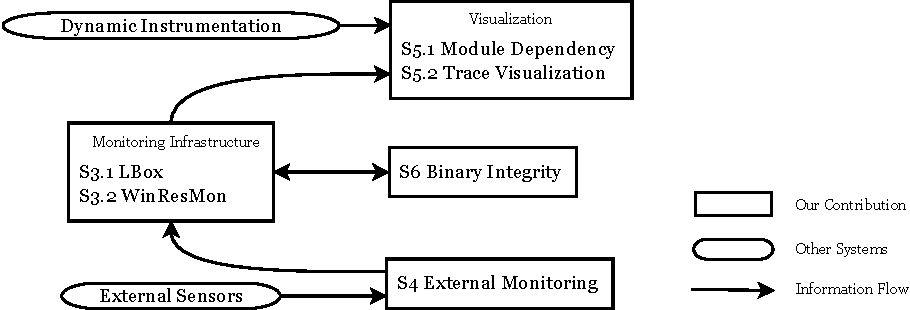
\includegraphics[width=1.0\textwidth]{overview.pdf}
\caption{Overview of the Contributions}
\label{fig:overview}
\end{figure}

Figure~\ref{fig:overview} visualizes the contributions and relationships between
the work in this thesis.
The monitoring infrastructures serve as the base in our research.
Traces collected by the monitoring infrastructure along with other information is used
in various visualizations.
External sensors gather information which is used to manage and control resources within and outside
a host machine in our external monitoring work.
The monitoring infrastructure records the binary related information flow
which is used in our binary integrity security model.

Many parts of the thesis are demonstrated in Windows with system prototypes because of the great
variety of software and number of users which attract many attacks.
The closed source nature also makes the monitoring challenging and
demanding.
However, the ideas can be applied on other operating systems.

The published works included in this thesis are listed below in
chronological order.

\begin{tightenumerate}
\item
Yongzheng Wu and Roland H.C. Yap.
\newblock A user-level framework for auditing and monitoring.
\newblock In {\em Proceedings of the 21st Annual Computer Security Applications
  Conference (ACSAC'05)}, pages 95--105. IEEE Computer Society, 2005.
\newblock (in {\bf Section~\ref{sec:lbox}})

\item
Rajiv Ramnath, Rajiv Sufatrio, Roland H.C. Yap, and Yongzheng Wu.
\newblock WinResMon: a tool for discovering software dependencies,
  configuration and requirements in Microsoft Windows.
\newblock In {\em Proceedings of the 20th Conference on Large Installation
  System Administration (LISA'06)}, pages 175--186. USENIX Association, 2006.
\newblock (in {\bf Section~\ref{sec:winresmon}})

\item
Felix Halim, Rajiv Ramnath, Yongzheng Wu, and Roland H.C. Yap.
\newblock A lightweight binary authentication system for windows.
\newblock {\em Trust Management II}, pages 295--310, 2008.
\newblock (in {\bf Section~\ref{sec:binauth}})

\item
Yongzheng Wu, Sufatrio, Roland H.C. Yap, Rajiv Ramnath, and Felix Halim.
\newblock Establishing software integrity trust: A survey and lightweight
  authentication system for windows.
\newblock In Zheng Yan, editor, {\em Trust Modeling and Management in Digital
  Environments: from Social Concept to System Development}, chapter~3. IGI
  Global, 2009.
\newblock (in {\bf Section~\ref{sec:binauth}})

\item
Ee-Chien Chang, Liming Lu, Yongzheng Wu, Roland H. C. Yap, and Jie Yu.
\newblock Enhancing host security using external environment sensors.
\newblock In {\em Proceedings of the 6th International ICST Conference on
  Security and Privacy in Communication Networks (SecureComm 2010)}, volume~50,
  pages 362--379. Springer, 2010.
\newblock (in {\bf Chapter~\ref{sec:sensor}})

\item
Yongzheng Wu and Roland H.C. Yap.
\newblock The problem of usable binary authentication.
\newblock In {\em Proceedings of the 4th International Conference on Secure
  Software Integration and Reliability Improvement Companion (SSIRI'10)}, pages 34--35.
  IEEE Computer Society, 2010.
\newblock (in {\bf Section~\ref{sec:binint}})

\item
Yongzheng Wu, Roland H.C. Yap, and Felix Halim.
\newblock Visualizing Windows system traces.
\newblock In {\em Proceedings of the 5th International Symposium on Software
  visualization (SOFTVIS'10)}, pages 123--132. ACM, 2010.
\newblock (in {\bf Section~\ref{sec:lviz}})

\item
Yongzheng Wu, Roland H.C. Yap, and Rajiv Ramnath.
\newblock Comprehending module dependencies and sharing.
\newblock In {\em Proceedings of the 32nd ACM/IEEE International Conference on
  Software Engineering (ICSE'10)}, volume~2, pages 89--98. ACM, 2010.
\newblock (in {\bf Section~\ref{sec:depvis}})

\item
Yongzheng Wu and Roland H.C. Yap.
\newblock Towards a binary integrity system for Windows.
\newblock In {\em Proceedings of the 6th ACM Symposium on Information, Computer
  and Communications Security (ASIACCS'11)},
  pages 503--507. ACM, 2011.
\newblock (in {\bf Section~\ref{sec:binint}})

\item
Ee-Chien Chang, Liming Lu, Yongzheng Wu, Roland H. C. Yap, and Jie Yu.
\newblock Enhancing host security using external environment sensors.
\newblock In {\em Special Issue in Intentional Journal of Information Security (IJIS)},
  Springer, 2011. (to appear)
\newblock (in {\bf Chapter~\ref{sec:sensor}})
\end{tightenumerate}

The following are other published works by the author during
his doctoral candidature, that are not related to this thesis.

\begin{tightenumerate}
\item
Felix Halim, Yongzheng Wu and Roland H.C. Yap.
\newblock Security Issues in Small World Network Routing.
\newblock In {\em Proceedings of the 2nd IEEE International Conference on
  Self-Adaptive and Self-Organizing Systems (SASO 2008)},
  pages 493--494. IEEE Computer Society, 2008.

\item
Felix Halim, Yongzheng Wu and Roland H.C. Yap.
\newblock Small World Networks as (Semi)-Structured Overlay Networks.
\newblock In {\em Workshops Proceedings of the 2nd IEEE International
  Conference on Self-Adaptive and Self-Organizing Systems
  (SASO Workshops 2008)},
  pages 214--218. IEEE Computer Society, 2008.

\item
Felix Halim, Yongzheng Wu and Roland H.C. Yap.
\newblock Wiki credibility enhancement.
\newblock In {\em Proceedings of the 2009 International Symposium on Wikis (WikiSym'09)},
  pages 17:1--17:4. ACM, 2009.

\item
Felix Halim, Yongzheng Wu and Roland H.C. Yap.
\newblock Routing in the Watts and Strogatz Small World Networks Revisited.
\newblock In {\em Workshops Proceedings of the 4th IEEE International
  Conference on Self-Adaptive and Self-Organizing Systems
  (SASO Workshops 2010)},
  pages 247--250. IEEE Computer Society, 2010.

\item
Felix Halim, Roland H.C. Yap and Yongzheng Wu.
\newblock A MapReduce-Based Maximum-Flow Algorithm for Large Small-World
  Network Graphs.
\newblock In {\em Proceedings of the 2011 IEEE 31th International Conference on
  Distributed Computing Systems (ICDCS'11)},
  IEEE Computer Society, 2011.
\end{tightenumerate}

\section{Thesis Organization}
\label{sec:outline}

The rest of the thesis is organized as follows.
Chapter~\ref{sec:bg} gives some background knowledge on operating
system monitoring and Windows.
We also show and some existing monitoring systems and tools.
Chapter~\ref{sec:mon} presents our monitoring infrastructures LBox
and WinResMon.
Chapter~\ref{sec:sensor} shows our research on external monitoring.
Chapter~\ref{sec:vis} presents our two trace visualization works.
Chapter~\ref{sec:auth} shows the binary authentication system and
the binary integrity security model.
Finally, Chapter~\ref{sec:concl} concludes the thesis and points out
directions for future work.
